% !TeX root = ../main.tex

\chapter{相关背景介绍和相关工作对比}
本章先介绍单智能体强化学习,然后引入本项目用到的多智能强化学习的一种建模方式,之后介绍实验环境以及信息论相关的基本概念,最后给出和本项目相关的工作以及和本项目的区别。
\section{单智能体强化学习简介}
本节会简单介绍一些必须的单智能体强化学习知识,然后下一节讲述本文用到的多智能体强化学习的建模。

\subsection{MDP}
强化学习的智能体需要在与环境的交互中连续地做决定。而这个环境常常表示成Markov决策过程(Markov Decision Process, MDP). MDP定义为一个元组$(S,A,P,R,\gamma)$, 其中$S$和$A$分别表示状态和动作空间,$P:S\times A\to \Delta (S)$表示从状态$s\in S$采取某个动作$a\in A$后转移到$s'\in S$的概率,$R: S\times A\times S\to \mathbb{R}$是激励函数,表示智能体在这种转移的过程中获得的激励值,$\gamma$称为折扣值,表示智能体更加期待立即的激励而不是未来的激励。

在每个时刻$t$, 智能体面对的是系统的状态$s_t$, 然后做出一步动作$a_t$, 这会让系统转移到下一个环境$s_{t+1}\sim P(\cdot|s_t,a_t)$. 除此之外,智能体还会收到一个及时的激励$R(s_t,a_t,s_{t+1})$. 解决这个MDP的目标就是找到一个策略$\pi:S\to \Delta(A)$, 即一个从状态空间$S$到动作空间$A$的映射,也就是动作$a_t\sim \pi(\cdot|s_t)$, 最终的折扣后的累计激励为
\begin{equation}
    \mathbb{E}\left[\sum_{t\ge 0}\gamma^t R(s_t,a_t,s_{t+1})\bigg|a_t\sim\pi(\cdot|s_t),s_0    \right]
\end{equation}
相应地,可以定义在策略$\pi$下的Q函数和值函数:
\begin{align}
Q_\pi(s,a) &= \mathbb{E}\left[\sum_{t\ge 0}\gamma^t R(s_t,a_t,s_{t+1})\bigg|a_t\sim\pi(\cdot|s_t),a_0=a,s_0 =s\right] \\
V_\pi(s) &= \mathbb{E}\left[\sum_{t\ge 0}\gamma^t R(s_t,a_t,s_{t+1})\bigg|a_t\sim\pi(\cdot|s_t),s_0 =s\right]
\end{align}

\subsection{基于值函数的方法}
基于值函数的方法需要找到一个对Q函数的好的估计,比如最优Q函数$Q_{\pi^*}$, 然后每一步的动作就可以选取让这个Q值最大的$a$. 一个非常著名的基于值函数的算法是Q-Learning, 在这个算法里,智能体会维护一个Q值的估计$\hat{Q}(s,a)$. 当从状态$s$由动作$a$转移到下一状态$s'$时,智能体会收到一个激励$r$, 然后按照如下方式更新Q函数:
\begin{equation}
    \hat{Q}(s,a)\leftarrow (1-\alpha)\hat{Q}(s,a) + \alpha \left[ r + \gamma \max_{a'}\hat{Q}(s',a') \right]
\end{equation}
这里的$\alpha>0$是学习速率。

\subsection{基于策略函数的方法}
另一类方法是直接在策略函数空间搜索,通常这个策略函数用神经网络来估计,也就是$\pi_\theta(\cdot|s)\approx \pi(\cdot|s)$. 所以,最直接的方法就是好沿着增大累加激励的方向更新策略函数,也就是策略梯度方法:
\begin{equation}
    \nabla J(\theta) = \mathbb{E}_{a\sim \pi_{\theta}(\cdot|s),s\sim\eta_{\pi_\theta}(\cdot)}\left[Q_{\pi_\theta}(s,a)\nabla \log \pi_\theta (a|s) \right]
\end{equation}
其中,$J(\theta)$是期望返回值,$Q_{\pi_\theta}$是在策略$\pi_\theta$下的Q函数,$\eta_{\pi_\theta}$是状态出现的频率。

\section{多智能体强化学习简介}
和单智能体强化学习类似,MARL也是考虑解决一个连续的决定问题,但是有多个智能体参与进来。具体来说,整个环境系统的演化和智能体收到的激励都会受到所有智能体的动作构成的联合动作的影响。

本项目考虑一个完全协作的多智能体任务,这可以被建模成Dec-POMDP, 也就是~\cite{oliehoek2016concise}$G=\langle I, S, A, P, R, \Omega, O, n, \gamma\rangle$, 其中$A$是有限的动作空间, $I\equiv\{1,2,...,n\}$是有限的智能体集合, $\gamma\in[0, 1)$是discount factor,$s\in S$是环境真正的状态。这里考虑一个部分可观测的环境,智能体$i$只能观测到$o_i\in \Omega$, 这个观测来自观测函数$O(s, i)$. 每个智能体有个历史轨迹$\tau_i\in \Tau\equiv(\Omega\times A)^*$. 每个时间步,每个智能体$i$会选择一个动作$a_i\in A$, 和其他所有智能体的动作联合形成一个联合动作$\va$ $\in A^n$,然后根据转移函数$P(s'|s, \va)$会得到下一个状态$s'$,以及一个共享的激励$r=R(s,\va)$.联合策略函数$\bm{\pi}$能推导出一个联合的动作-值函数$Q_{tot}^{\bm{\pi}}(s,\va)=\mathbb{E}_{s_{0:\infty},\va_{0:\infty}}[\sum_{t=0}^\infty \gamma^{t}r_t|s_0=s,\va_0=\va,\bm{\pi}]$. 

为了更高效地学习智能体的策略,集中训练、分离执行(Centralized Training with Decentralized Execution (CTDE)~\cite{foerster2016learning, foerster2018counterfactual}广泛应用。一种很有前景的利用CTDE的方式是值函数分解~\cite{sunehag2018value, rashid2018qmix, son2019qtran}, 简要来说就是每个智能体学习一个分离的局部效用函数(Local Utility Function),然后用一个混合网络来结合这些局部的值,输出全局的动作-值信息。本项目也是利用CTDE框架,与之前的算法不同的是,局部效用函数不是完全共享的,也不是完全各自独立的,而是在相似角色的智能体之间共享,对不相似角色来说是分离的。

\section{星际争霸II实验环境简介}
星际争霸II\footnote{StarCraft II are trademarks of Blizzard Entertainment\textsuperscript{TM}.} 单元微操作任务~\cite{samvelyan2019starcraft}被认为是最具挑战性的协同多智能体基准测试环境,因为它有很高的控制复杂度和环境随机性。其框架\footnote{\url{https://github.com/oxwhirl/pymarl}}基于PyTorch实现,可以开源获取。

许多算法\cite{foerster2017stabilising, foerster2018counterfactual, rashid2018qmix, mahajan2019maven}都是使用该环境训练测试的,本项目也是如此,图\ref{fig:starcraft2-MMM2}为本项目在星际争霸II其中一个地图MMM2的回放的截图。

\begin{figure}[htb]
    \centering
    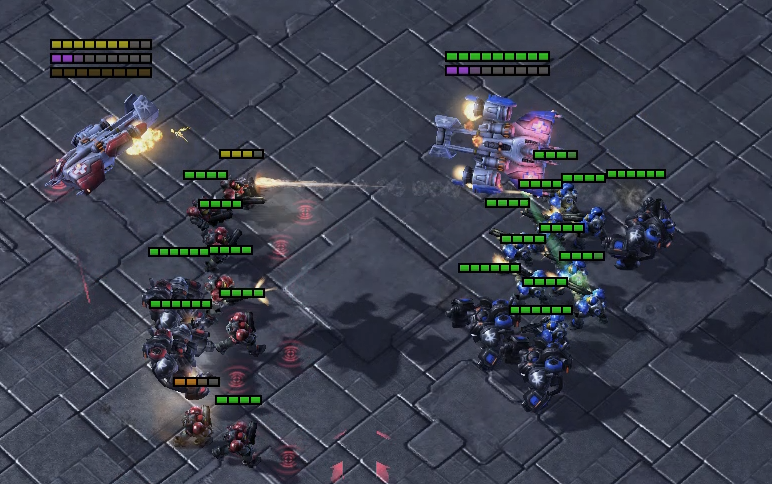
\includegraphics[width=0.8\textwidth]{figures/common/starcraft2-MMM2.png}
    \caption{星际争霸II 地图MMM2}
    \label{fig:starcraft2-MMM2}
  \end{figure}


星际争霸主要有两个层面的操作,宏操作和微操作,其中宏操作是指高阶的策略考虑,比如经济和资源的管理。pymarl框架主要关注的问题是星际争霸II中的微操作问题,也就是控制低阶的一些操作,比如在智能体对抗敌人的时候,控制我方智能体的移动和攻击等等。这种方式让这个环境天然地适合多智能体系统,因为每个星际争霸的单元可以用一个分离的控制器来代替,而敌方的单元则是用星际争霸自己人工写的策略来控制。

智能体得到的激励是共享的同一个,根据攻击敌人、自身受伤、敌方死亡、本局胜负的一个线性函数来确定。智能体效用函数的输入是局部的观测,混合函数的超网络的输入包括了全局的观测。局部观测是一个很小的区域范围,能观测到这个范围内的其他智能体的信息,比如距离、相对坐标、血量、护盾值、类型。全局观测仅仅是给混合网络的超网络,只能在集中训练的时候能获取,在测试的时候没有。它包括所有智能体相对地图中心的坐标、智能体的特性向量(和局部观测一致). 智能体的动作空间是离散的,包括移动(东南西北)、攻击(某个敌人)、停止、空操作(死掉的智能体只能是空操作)。

对智能体合适的控制,能最小化自身的伤害而最大化对敌人的伤害。一个很有用的策略称之为集中火力(focus fire), 意思是控制我方所有的智能体集中攻击一个敌人,直到杀死它,然后换下一个。这样的好处是,能有效减少敌人的攻击力量,避免出现那些只有丝血但是仍然能全力开火的敌人。另外一些很重要的技巧包括,按照智能体的护甲类型来组织站位、和近战的敌人保持一定的距离而从远程攻击它、从不同的方向攻击敌人而让它左右往返耗费时间等等。本项目的某些实验回放可以看到智能体利用了这里的某些技巧。

\section{信息论基本概念简介}
\subsection{熵}
在信息论里面,熵的作用是用来衡量一个随机事件或者随机变量的不确定性的。

\subsubsection{自信息和熵}
自信息表示一个随机事件的信息量,一个随机事件发生的概率越高,它的自信息越低。
对于一个随机变量$X\in \mathcal{X}$, 概率分布为$P(x),x\in\mathcal{X}$, 当$X=x$时,自信息定义为
\begin{equation}
    I(x) = -\log p(x)
\end{equation}
而$X$的熵定义为自信息的期望,也就是
\begin{equation}
    H(X) = \mathbb{E}_X[I(x)] = \mathbb{E}_X[-\log p(x)]=-\int_{x\in\mathcal{X}}p(x)\log p(x)\mathrm{d}x
\end{equation}
可以发现,熵最大时,混乱程度最高,比如均匀分布。

\subsubsection{联合熵和条件熵}
将单个变量的熵推广到多个随机变量就是联合熵
\begin{equation}
    H(X,Y) = -\iint_{x\in\mathcal{X},y\in\mathcal{Y}}p(x,y)\log p(x,y)\mathrm{d}x\mathrm{d}y
\end{equation}
而条件熵为
\begin{equation}
    H(Y|X)=\int_{x\in\mathcal{X}}p(x)H(Y|X=x)\mathrm{d}x=-\iint_{x\in\mathcal{X},y\in\mathcal{Y}}p(x,y)\log p(y|x)\mathrm{d}x\mathrm{d}y
\end{equation}

\subsection{互信息}
\subsubsection{互信息}
互信息衡量两个随机变量相互包含的信息量。
\begin{equation}
    I(X;Y)=\iint_{x\in\mathcal{X},y\in\mathcal{Y}}p(x,y)\frac{p(x,y)}{p(x)p(y)}\mathrm{d}x\mathrm{d}y
\end{equation}
有一条很重要的性质是
\begin{equation}
    I(X;Y)=H(X)-H(X|Y)=H(Y)-H(Y|X)
\end{equation}
如果两个随机变量独立,即$p(x,y)=p(x)p(y)$, 则它们之间的互信息为0.

\subsubsection{条件互信息}
条件互信息是指,在给定$Z$时,由于$Y$的知识而引起的$X$的不确定度的减少。
\begin{equation}
    I(X;Y|Z)=H(X|Z)-H(X|Y,Z)=\iiint_{x\in\mathcal{X},y\in\mathcal{Y},z\in\mathcal{Z}}p(x,y,z)\frac{p(x,y|z)}{p(x|z)p(y|z)}\mathrm{d}x\mathrm{d}y\mathrm{d}z
\end{equation}


\subsection{交叉熵和散度}
\subsubsection{交叉熵}
对于分布为$p(x)$的随机变量,熵$H(X)$表示起最优的编码长度,交叉熵是按照概率分布$q$对$p$的信息进行编码时的编码长度
\begin{equation}
    H(p,q)=\mathbb{E}_{p}[-\log q(x)]= -\int_{x\in\mathcal{X}}p(x)\log q(x)\mathrm{d}x
\end{equation}
可以用来衡量两个分布的接近程度

\subsubsection{KL散度}
也称为相对熵,表示用概率分布$q$来近似$p$时所造成的信息损失量,
\begin{equation}
    \KL(p\|q)=H(p,q)-H(p)=\int_{x\in\mathcal{X}}p(x)\log \frac{p(x)}{q(x)}\mathrm{d}x
\end{equation}
注意$\KL(p\|q)\ge 0$, 当且仅当$p=q$时等号成立。


条件相对熵定义为
\begin{equation}
    \KL(p(y|x)\|q(y|x))=\iint_{x\in\mathcal{X},y\in\mathcal{Y}}p(x,y)\log \frac{p(y|x)}{q(y|x)}\mathrm{d}x\mathrm{d}x
\end{equation}


\section{相关工作与对比}
角色的涌现已经在很多文献中有记录了,比如蜜蜂~\cite{jeanson2005emergence}, 蚂蚁~\cite{gordon1996organization}, 人类~\cite{butler2012condensed}等等。在这些系统中,角色和分工紧密相连,并且对提升劳动效率有很大的作用。同时,很多的多智能体系统受到了这些自然界的系统的启发。它们会分解任务,让有相同角色的智能体专注于某个子任务,以此来降低设计的复杂度~\cite{wooldridge2000gaia, omicini2000soda, padgham2002prometheus, pavon2003agent, cossentino2005passi, zhu2008role, spanoudakis2010using, deloach2010mase, bonjean2014adelfe}. 但这些方法都被设计用于有清晰结构的任务,比如软件工程~\cite{bresciani2004tropos}. 因此,它们会预定义角色以及相关的子任务~\cite{ Lhaksmana2018role}。与之不同的是,本框架是隐式地把角色概念引入多智能体的连续决定,并且环境是动态和未知的。

深度多智能体强化学习在近几年有很大的进步。COMA~\citep{foerster2018counterfactual}, MADDPG~\citep{lowe2017multi}, PR2~\citep{wen2019probabilistic}, 和MAAC~\cite{iqbal2019actor}集中注意力在多智能体的策略梯度方法。另一条主线是关注基于值函数的多智能体强化学习, VDN~\citep{sunehag2018value}, QMIX~\citep{rashid2018qmix}, 和 QTRAN~\citep{son2019qtran}依次扩大了混合网络能表达的函数的范围。另一方面,涌现也是一个在深度多智能体强化学习逐渐引起重视的话题,相关的工作有交流的涌现~\cite{foerster2016learning, lazaridou2017multi, das2017learning, mordatch2018emergence}, 公平性的涌现~\cite{jiang2019learning}, 工具使用的涌现~\cite{baker2020emergent}, 这些涌也提供了一个用深度学习理解自然或者人工多智能体系统的新角度。

为了学到多样化以及可识别的角色,本算法提出优化关于个人角色和轨迹的互信息,最近的一个研究多智能体探索的算法MAVEN~\cite{mahajan2019maven}也用了类似的目标函数。但是不同的是,MAVEN的目标是集体的探索,这是在高层次思想的不同,同样也造成了很多技术细节的不同。除此之外,在实验章节,也比较了本算法与MAVEN的性能不同。

\section{本章小结}
本章先简单介绍了单智能体强化学习的背景,然后着重介绍本文所用的多智能体强化学习的建模,进一步介绍了本项目所采用的实验环境星际争霸II,以及给出一些信息论相关的简介,最后给出了与本文相关的工作,以及本项目与之的不同。
